%% This includes day 2 Concepts
\documentclass[12pt,a4paper]{article}

\usepackage{graphicx}

% For mathematical equations
\usepackage{amsmath}

\usepackage{enumitem}% For changing the enumerate item
%opening
\title{India}
\author{Wikipedia}
%\date{June 29,2020}


\begin{document}

\maketitle
\tableofcontents
\listoffigures
\listoftables


\section{Introduction}
%justified by default
\paragraph{}
\textbf{India} accounts for the bulk of the Indian subcontinent, lying atop the
Indian tectonic plate, a part of the Indo-Australian Plate. India’s 
defining geological processes began \underline{75 million }years ago when the Indian Plate, 
then part of the southern supercontinent Gondwana, began a
north-eastward drift caused by seafloor spreading to its south-west, and
later, south and south-east.

% Left aligned 
\begin{flushleft}
Simultaneously, the vast Tethyan oceanic
crust, to its northeast, began to subduct under the Eurasian Plate.These
dual processes, driven by convection in the Earth’s mantle, both cre
ated the Indian Ocean and caused the Indian continental crust even
tually to under-thrust Eurasia and to uplift the Himalayas.Immediately
south of the emerging \textbf{Himalayas}, plate movement created a vast trough
that rapidly filled with river-borne sediment and now constitutes the
Indo-Gangetic Plain. Cut off from the plain by the ancient \textit{Aravalli
Range} lies the \textit{Thar Desert}.
\end{flushleft}


\subsection{History}
\paragraph{}
By 55,000 years ago, the first modern humans had arrived on the Indian
subcontinent from Africa, where they had earlier evolved. The earli
est known modern human remains in South Asia date to about 30,000
years ago.After 6500 BCE, evidence for domestication of food crops
and animals, construction of permanent structures, and storage of agri
cultural surplus appeared in Mehrgarh and other sites in what is now
Balochistan.These gradually developed into the Indus Valley Civili
sation,the first urban culture in South Asia, which flourished during
2500–1900 BCE in what is now Pakistan and western India.
%Right Aligned
\begin{flushright}
	India accounts for the bulk of the Indian subcontinent, lying atop the Indian tectonic plate, a part of the Indo-Australian Plate. India's defining geological processes began 75 million years ago when the Indian Plate, then part of the southern supercontinent Gondwana, began a north-eastward drift caused by seafloor spreading to its south-west, and later, south and south-east. Simultaneously, the vast Tethyan oceanic crust, to its northeast, began to subduct under the Eurasian Plate.These dual processes, driven by convection in the Earth's mantle, both created the Indian Ocean and caused the Indian continental crust eventually to under-thrust Eurasia and to uplift the Himalayas.[161] Immediately south of the emerging Himalayas, plate movement created a vast trough that rapidly filled with river-borne sediment and now constitutes the Indo-Gangetic Plain. Cut off from the plain by the ancient Aravalli Range lies the Thar Desert.
\end{flushright}

\section{Government}

The Government of India comprises three branches:
\begin{itemize}
	\item Executive: The President of India is the ceremonial head of state, who is elected indirectly for a five-year term by an electoral college comprising members of national and state legislatures. The Prime Minister of India is the head of government and exercises most executive power.Appointed by the president, the prime minister is by convention supported by the party or political alliance having a majority of seats in the lower house of parliament. The executive of the Indian government consists of the president, the vice president, and the Union Council of Ministers—with the cabinet being its executive committee—headed by the prime minister. Any minister holding a portfolio must be a member of one of the houses of parliament. In the Indian parliamentary system, the executive is subordinate to the legislature; the prime minister and their council are directly responsible to the lower house of the parliament. Civil servants act as permanent executives and all decisions of the executive are implemented by them.
	\item Legislature: The legislature of India is the bicameral parliament. Operating under a Westminster-style parliamentary system, it comprises an upper house called the Rajya Sabha (Council of States) and a lower house called the Lok Sabha (House of the People). The Rajya Sabha is a permanent body of 245 members who serve staggered six-year terms. Most are elected indirectly by the state and union territorial legislatures in numbers proportional to their state's share of the national population. All but two of the Lok Sabha's 545 members are elected directly by popular vote; they represent single-member constituencies for five-year terms.[240] The remaining two members are nominated by the president from among the Anglo-Indian community, in case the president decides they are not adequately represented.
	\item Judiciary: India has a three-tier unitary independent judiciary comprising the supreme court, headed by the Chief Justice of India, 25 high courts, and a large number of trial courts. The supreme court has original jurisdiction over cases involving fundamental rights and over disputes between states and the centre and has appellate jurisdiction over the high courts. It has the power to both strike down union or state laws which contravene the constitution, and invalidate any government action it deems unconstitutional.
\end{itemize}
\subsection{Administrative Divisions}
There are 28 states and 8 Union Territories
\begin{itemize}
	\item States
	\begin{enumerate}
		\item Andhra Pradesh
		\item Arunachal Pradesh
		\item Assam
		\item Bihar
		\item Chhattisgarh
		\item Goa
		\item Gujarat
		\item Haryana
		\item Himachal Pradesh
		\item Jharkhand
		\item Karnataka
		\item Kerala
		\item Madhya Pradesh
		\item Maharashtra
		\item Manipur
		\item Meghalaya
		\item Mizoram
		\item Nagaland	
	\end{enumerate}
	\item Union Territories
	\begin{enumerate}[label= (\Alph*)]
		\item Andaman and Nicobar Islands
		\item Chandigarh
		\item Dadra and Nagar Haveli and Daman and Diu
		\item Jammu and Kashmir
		\item Ladakh
		\item Lakshadweep
		\item National Capital Territory of Delhi
		\item Puducherry
	\end{enumerate}
\end{itemize}

\newpage
\section{National and Official Symbols of India}
\subsection{Flag of India}
The National Flag of India as shown in \textbf{fig}.\ref{fig:flag} is a horizontal rectangular tricolour of India saffron, white and India green; with the Ashoka Chakra, a 24-spoke wheel, in navy blue at its centre. It was adopted in its present form during a meeting of the Constituent Assembly held on 22 July 1947, and it became the official flag of the Dominion of India on 15 August 1947. The flag was subsequently retained as that of the Republic of India. In India, the term "tricolour" almost always refers to the Indian national flag. The flag is based on the Swaraj flag, a flag of the Indian National Congress designed by Pingali Venkayya.

By law, the flag is to be made of khadi, a special type of hand-spun cloth or silk, made popular by Mahatma Gandhi. The manufacturing process and specifications for the flag are laid out by the Bureau of Indian Standards. The right to manufacture the flag is held by the Khadi Development and Village Industries Commission, who allocates it to regional groups. As of 2009, the Karnataka Khadi Gramodyoga Samyukta Sangha has been the sole manufacturer of the flag.

\begin{figure}[h]
	\centering
	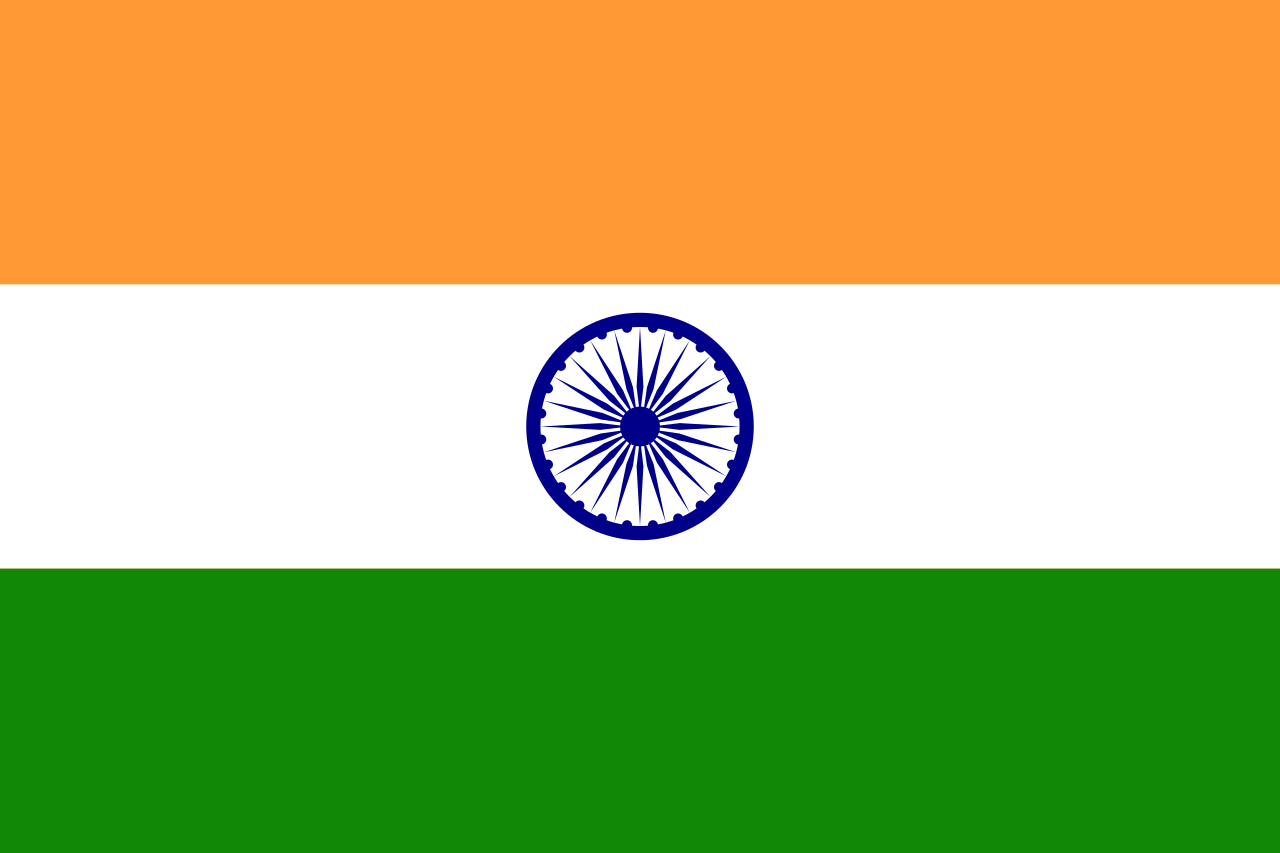
\includegraphics[width = 0.7\linewidth]{../Images/flag}	
	\caption[National Flag]{Tricoloured Indian National Flag}
	\label{fig:flag}
\end{figure}

\subsection{National Motto}
"Satyameva Jayate" - "Truth alone triumphs" is a part of a mantra from the Hindu scripture Mundaka Upanishad.Following the independence of India, it was adopted as the national motto of India on 26 January 1950, the day India became a republic. It is inscribed in the Devanagari script at the base of the Lion Capital of Ashoka and forms an integral part of the Indian national emblem as shown in fig.\ref{fig:emblem}. The emblem and the words "Satyameva Jayate" are inscribed on one side of all Indian currency and national documents.


\begin{figure}[h]
	\centering
	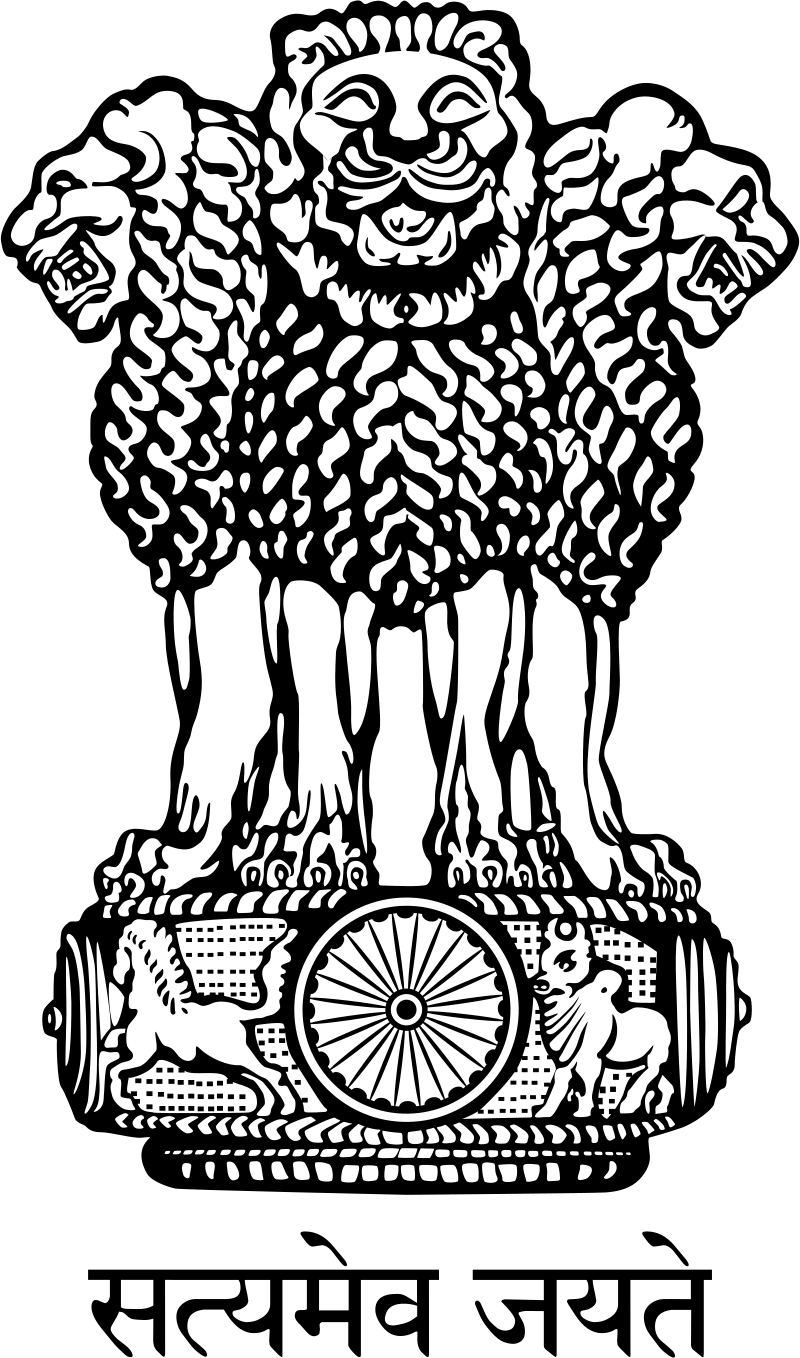
\includegraphics[width= 0.3\linewidth,height=0.3\linewidth]{../Images/emblem}
	\caption[National Emblem]{National Emblem of India contains the phrase Satyameva Jayate}
	\label{fig:emblem}
\end{figure}


\section{Vital Statistics}

\begin{table}[h]
	\centering
	\begin{tabular}{|c|c|c|c|c|c|c|}
		\hline
		State & \multicolumn{3}{|c|}{Birth Rate}&\multicolumn{3}{|c|}{Natural growth Rate}\\
		\cline{2-7}
		& Total & Rural & Urban &Total & Rural & Urban\\
		\hline
		Karnataka & 19.2 &	20.2 &	17.5 &12.1	&12.1&	12.1\\
		\hline
		Delhi &	17.8 & 	19.7	&17.5	&13.6&	15.0	&13.4\\
		\hline
		Tamil Nadu	&15.9&	16.0&	15.8	&8.3	&7.8	&8.9\\
		\hline
		Kerala&	14.8&	14.8&	14.8& 7.8&	7.7	&8.1\\
		\hline		
	\end{tabular}
	\caption[Vital Statistics]{Regional Vital Statistics By State }
	\label{table:statistics}
\end{table}


\section{Indian Mathematics}
Indian mathematics emerged in the Indian subcontinent from 1200 BC until the end of the 18th century. In the classical period of Indian mathematics (400 AD to 1200 AD), important contributions were made by scholars like Aryabhata, Brahmagupta, Bhaskara II, and Varāhamihira. The decimal number system in use today was first recorded in Indian mathematics. Indian mathematicians made early contributions to the study of the concept of zero as a number, negative numbers, arithmetic, and algebra. In addition, trigonometry was further advanced in India, and, in particular, the modern definitions of sine and cosine were developed there. These mathematical concepts were transmitted to the Middle East, China, and Europe[7] and led to further developments that now form the foundations of many areas of mathematics.
\subsection{Sulba Sutras}

Baudhayana (c. 8th century BCE) composed the Baudhayana Sulba Sutra, the best-known Sulba Sutra, which contains examples of simple Pythagorean triples, such as: $(3, 4, 5), (5, 12, 13), (8, 15, 17), (7, 24, 25),\text{and }  (12, 35, 37)$ as well as a statement of the Pythagorean theorem for the sides of a square: "The rope which is stretched across the diagonal of a square produces an area double the size of the original square."[29] It also contains the general statement of the Pythagorean theorem (for the sides of a rectangle): "The rope stretched along the length of the diagonal of a rectangle makes an area which the vertical and horizontal sides make together."Baudhayana gives a formula for the square root of two as show in \eqref{sqroot}:
\begin{equation}
\sqrt{2} \approx 1+ \frac{1}{3} + \frac{1}{ 3 \cdot 4} - \frac{1}{3 \cdot 4 \cdot 34} = 1.4142156\dots
\label{sqroot}
\end{equation}

\subsection{Pingala (300 BCE – 200 BCE)}
Among the scholars of the post-Vedic period who contributed to mathematics, the most notable is Pingala , a music theorist who authored the Chhandas Shastra , a Sanskrit treatise on prosody.  

The text also indicates that Pingala was aware of the combinatorial identity. The equation is shown in \eqref{cidentity}\\

\begin{equation}
\binom{n}{0} + \binom{n}{1} +\binom{n}{2} +\dots  +\binom{2}{n+1} + \binom{n}{n} = 2^n
\label{cidentity}
\end{equation}


\subsection{Jain Mathematics}
Although Jainism is a religion and philosophy predates its most famous exponent, the great Mahaviraswami (6th century BCE), most Jain texts on mathematical topics were composed after the 6th century BCE. Jain mathematicians are important historically as crucial links between the mathematics of the Vedic period and that of the "classical period."

A significant historical contribution of Jain mathematicians lay in their freeing Indian mathematics from its religious and ritualistic constraints. In particular, their fascination with the enumeration of very large numbers and infinities led them to classify numbers into three classes: enumerable, innumerable and infinite. Infinity in mathematics is represented by $\infty$

\section{Inserting References}
There are three references included in the references.bib for demonstration purpose only . Those are cited as \cite{vanet},\cite{adhoc1}, \cite{xmpp}.

\bibliographystyle{ieeetr}

\addcontentsline{toc}{section}{References}
\bibliography{references.bib}

\section*{Disclaimer}
All the contents which are incorporated in this document are with the intentions to learn documentation using \LaTeX. All the information including tables figures and data sheets are taken from wikipedia. 


\end{document}
